\documentclass[varwidth=\maxdimen]{standalone}
\usepackage{pgfplots}
\usepackage{pgfplotstable}
\usepackage{tikz}
\usetikzlibrary{
  decorations.pathreplacing,
  calc,
  decorations.fractals,
  through,
  shapes,
  patterns,
  arrows.meta,
  arrows,
  calligraphy,
  shapes.symbols,
  shapes.geometric,
  patterns,
  matrix,
  fit
}
\usepackage{amsmath}
\usepackage{amsfonts}
\usepackage{xfrac}
\usepackage{xcolor}
% \usepackage{xr}
\usepackage{mathtools}
\usepackage{xr-hyper}
\usepackage{hyperref}
\externaldocument{Invariant_Measure_SHE_JPT_Revision}
\newcommand\R{\mathbb{R}}

\begin{document}

\colorlet{contrast_color_1}{gray!20!black}
\colorlet{contrast_color_2}{gray!70!black}

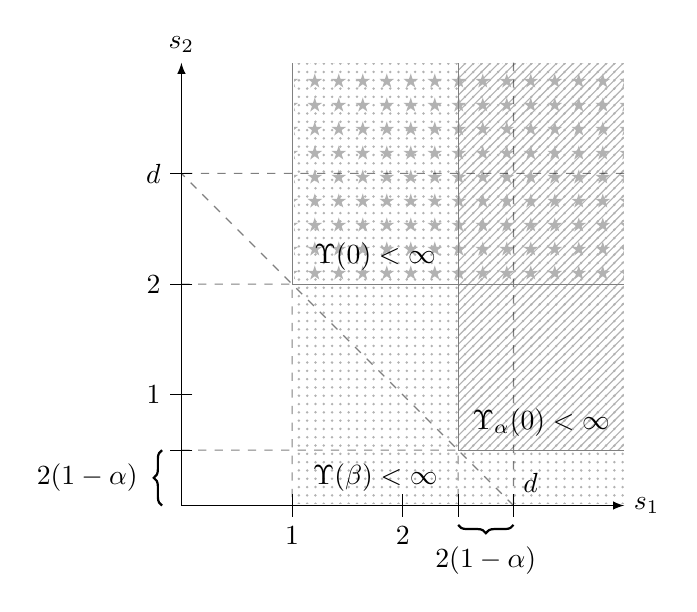
\begin{tikzpicture}[scale=1, transform shape, x = 4em, y = 4em]
  \tikzset{>=latex}


  \filldraw[draw = white, pattern color = black!30, pattern=fivepointed stars] (1,4) -- (1,2) -- (4,2) -- (4,4) -- cycle;
  \filldraw[draw = white, pattern color = black!30, pattern=north east lines] (2.5,4) -- (2.5,0.5) -- (4,0.5) -- (4,4) -- cycle;
  \filldraw[draw = white, pattern color = black!30, pattern = dots] (1.01,0.01) -- (1.01,4) -- (4,4) -- (4,0.01) -- cycle;

  \draw[dashed, opacity = 0.5] (3,0) -- (0,3) (3,4) -- (3,0) (4,3) -- (0,3) (0,2) -- (1,2) -- (1,0) (0,0.5) -- (2.5,0.5) -- (2.5,0);

  \draw[->] (0,0) -- (4,0) node[right] {$s_1$};
  \draw[->] (0,0) -- (0,4) node[above] {$s_2$};
  \draw (3,0.1) --++(0,-0.2) node[above right, yshift = 5pt] {$d$};
  \draw (2,0.1) --++(0,-0.2) node[below] {$2$};
  \draw (1,0.1) --++(0,-0.2) node[below] {$1$};
  \draw (2.5,0.1) --++(0,-0.2);

  \draw (0.1,3) --++(-0.2,0) node[left] {$d$};
  \draw (0.1,2) --++(-0.2,0) node[left] {$2$};
  \draw (0.1,1) --++(-0.2,0) node[left] {$1$};
  \draw (0.1,0.5) --++(-0.2,0);

  \draw[color = gray]
    (1,2) --++ (0,2)
    (2.5, 0.5)--++(0,3.5)
    (1,2) --++ (3,0)
    (2.5, 0.5)--++(1.5,0);
  \node[] (Upsilon0infty) at (1.75,2.25) {$\Upsilon(0)<\infty$};
  \node[] (Upsilonalpha0infty) at (3.25,0.75) {$\Upsilon_\alpha(0)<\infty$};
  \node[] (Upsilonalpha0infty) at (1.75,0.25) {$\Upsilon(\beta)<\infty$};

  \draw[decorate, thick, decoration = {brace, amplitude=3pt, raise=7pt}] (0,0) -- (0,0.5) node[midway, xshift = -3.4em] {$2(1-\alpha)$};
  \draw[decorate, thick, decoration = {brace, amplitude=3pt, raise=7pt}] (3,0) -- (2.5,0) node[midway, yshift = -2em] {$2(1-\alpha)$};
  % \draw[decorate, decoration = {calligraphic brace, amplitude=5pt, raise=5pt}] (0,0) -- (0,0.5);
\end{tikzpicture}
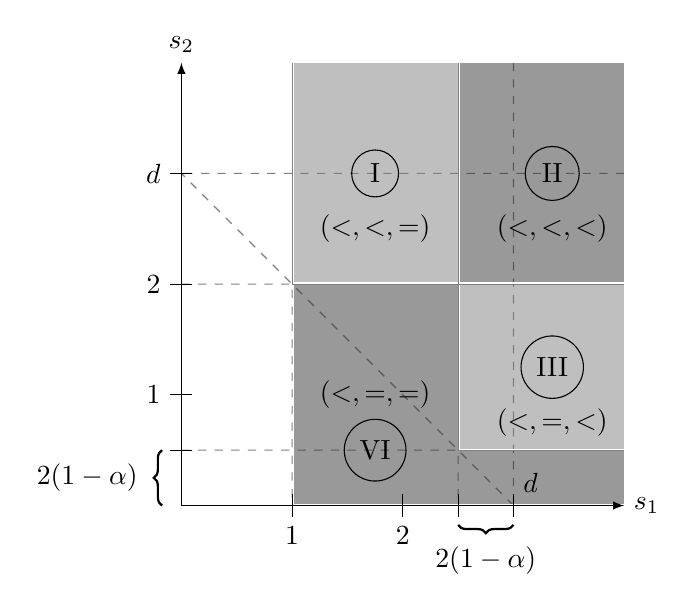
\begin{tikzpicture}[scale=1, transform shape, x = 4em, y = 4em]
  \tikzset{>=latex, node distance = 2em}

  \draw[dashed, opacity = 0.5] (3,0) -- (0,3) (3,4) -- (3,0) (4,3) -- (0,3) (0,2) -- (1,2) -- (1,0) (0,0.5) -- (2.5,0.5) -- (2.5,0);

  \filldraw[fill = black!50!white, fill opacity=0.5, draw = white] (1.01,4) -- (1.01,2.01) -- (2.5,2.01) -- (2.5,4) -- cycle; \node[draw, circle] (a) at (1.75,3) {I};  \node [below of = a] {$(<,<,=)$};
  \filldraw[fill = black!80!white, fill opacity=0.5, draw = white] (2.51,4) -- (2.51,2.01) -- (4,2.01) -- (4,4) -- cycle;     \node[draw, circle] (a) at (3.35,3) {II}; \node [below of = a] {$(<,<,<)$};
  \filldraw[fill = black!50!white, fill opacity=0.5, draw = white] (2.51,2) -- (2.51,0.51) -- (4,0.51) -- (4,2) -- cycle;     \node[draw, circle] (a) at (3.35,1.25) {III}; \node [below of = a] {$(<,=,<)$};
  \filldraw[fill = black!80!white, fill opacity=0.5, draw = white] (1.01,2) -- (1.01,0.01) -- (4,0.01) -- (4,0.5) -- (2.5,0.5) -- (2.5,2) -- cycle; \node[draw, circle] (a) at (1.75,0.5) {VI}; \node [above of = a] {$(<,=,=)$};

  \draw[->] (0,0) -- (4,0) node[right] {$s_1$};
  \draw[->] (0,0) -- (0,4) node[above] {$s_2$};
  \draw (3,0.1) --++(0,-0.2) node[above right, yshift = 5pt] {$d$};
  \draw (2,0.1) --++(0,-0.2) node[below] {$2$};
  \draw (1,0.1) --++(0,-0.2) node[below] {$1$};
  \draw (2.5,0.1) --++(0,-0.2);

  \draw (0.1,3) --++(-0.2,0) node[left] {$d$};
  \draw (0.1,2) --++(-0.2,0) node[left] {$2$};
  \draw (0.1,1) --++(-0.2,0) node[left] {$1$};
  \draw (0.1,0.5) --++(-0.2,0);

  \draw[color = gray]
    (1,2) --++ (0,2)
    (2.5, 0.5)--++(0,3.5)
    (1,2) --++ (3,0)
    (2.5, 0.5)--++(1.5,0);
  % \node[] (Upsilon0infty) at (1.75,2.25) {$\Upsilon(0)<\infty$};
  % \node[] (Upsilonalpha0infty) at (3.25,0.75) {$\Upsilon_\alpha(0)<\infty$};

  \draw[decorate, thick, decoration = {brace, amplitude=3pt, raise=7pt}] (0,0) -- (0,0.5) node[midway, xshift = -3.4em] {$2(1-\alpha)$};
  \draw[decorate, thick, decoration = {brace, amplitude=3pt, raise=7pt}] (3,0) -- (2.5,0) node[midway, yshift = -2em] {$2(1-\alpha)$};
  % \draw[decorate, decoration = {calligraphic brace, amplitude=5pt, raise=5pt}] (0,0) -- (0,0.5);
\end{tikzpicture}
\end{document}

